\documentclass[a4paper, 11pt]{article}
\usepackage[english]{babel}
\usepackage{appendix}
\input{"/media/alessandro/OS/Users/ale57/Documents/1. universita'/ANNO IV (2019-2020)/second semester/header.tex"}

\begin{document}

\title{NNDL Homework 3: \\ Deep Reinforcement Learning}
\author{Alessandro Lovo}
\maketitle

\section{Introduction}
  This homework will deal with Reinforcement learning using \emph{OpenAI}'s \emph{gym} environments. In particular we will start with the simple \emph{CartPole}, where the goal for the agent is to balance a pole on a cart, first providing the agent with high level knowledge of the environment, then giving it just the screen pixels. Then another gym environment will be tested. In every case the goal is to consistently beat the games with as few training episodes as possible.

  \subsection{General framework}
    The interaction between the environment and the agent and learning of the latter rely on the following framework of python classes and functions:
    \begin{itemize}
      \item \textbf{Policy net}: different architectures for deep neural networks taking as input the state of the environment and providing as output the Q-values for each possible actions.
      \item \textbf{Policy}: function for choosing which action to take given the Q-values and a generic parameter $\beta$. The possible policies are:
      \emph{random} (choose action randomly, ignoring the Q-values), \emph{greedy} (choose the action with the highest Q-value), \emph{$\epsilon$-greedy} (with probability $\epsilon$ choose a non optimal action, otherwise the greedy one; here $\beta$ is $\epsilon$), \emph{softmax} (here $\beta$ is the temperature parameter and the probability of choosing action $a$ is proportional to $e^{q_a/\beta}$). Both \emph{$\epsilon$-greedy} and \emph{softmax} policies reduce to the \emph{greedy} one whe $\beta = 0$.
      \item \textbf{Agent}: class for handling the interaction with the environment: it observes the state of the environment, passes it to the \emph{policy net} obtaining the Q-values, which uses, given a \emph{policy} to choose the action to take and pass back to the environment, receiving a reward and the next state.
      \item \textbf{Replay memory}: class containing a list of finite capacity with tuples [state, action, next state, reward] from which we randomly sample when training the agent. Once we reach the maximum capacity new data will overwrite the oldest ones.
      \item \textbf{Exploration profile}: class for scheduling the value of the $\beta$ parameter for the policy of the agent at every episode of training. Said value can either be predetermined, i.e. an exponential decay with the episode number, or depend on the current performance of the agent.
      \item \textbf{Evolver}: class for handling the training of the \emph{policy net} of the \emph{Agent}. It optimizes the smooth L1 loss between  $policy\_net(state, action)$ and $reward + \gamma \cdot target\_net(next\, state, best\, action)$ where $\gamma$ is the discount rate and the target net is a periodic checkpoint of the policy net. Data [state, action, next state, reward] are sampled from the \emph{replay memory} and the best action is computed using the greedy policy on the target net.
    \end{itemize}


\section{Cart-Pole}
  This environment consist of a cart able to move on a 1d rail with a pole attached, initially facing upwards. The state consists of four real numbers: cart position ($x$), cart velocity ($v$), pole angle ($\theta$), pole angular velocity ($\omega$) and the agent has two available actions: push the cart to the right or to the left. The game ends when the pole falls ($|\theta| > 12°$) or the cart goes out of screen ($|x| > 2.4$). The score of the agent is the number of steps until game termination and the game is considered beaten when the score reaches 500.

  I started testing a model that uses as policy net a fully connected network with [4, 128, 128, 2] neurons and hyperbolic tangent as activation function, with the softmax policy and trained with the SGD optimizer with learning rate $10^{-2}$ and a batch size of 128. Learning stops when the agent beats the game for 10 consecutive episodes.

  In the vanilla version at every step the agent receives a reward $r = 1$ until the pole falls, so the agent struggles to understand the consequence of its actions and learning is pretty slow and very dependent on the initialization of the net: running twice the learning with same hyperparameters can yield very different results. One of them is the one in fig \ref{fig:scores} (a) and an example of the behavior of the so trained agent is in \url{code/vanilla2.mp4}.

  To improve the results and speed up learning I proceeded in modifying the reward as $r = 1 + w_x |x|^{e_x} + w_\theta |\theta|^{e_\theta}$ basically suggesting to the agent that it needs to keep the pole vertical and the cart in the center of the screen.
  With the modified reward the results were better (fig \ref{fig:scores} (b) and \url{code/mod_r_cv.mp4} where the pole barely oscillates at all), but there was still a lot of margin for improvement in terms of learning speed.

  So I tried more exotic exploration profiles: for example a wavy profile (fig \ref{fig:scores} (c)) with the idea of having a region of low temperature quite early to see if the agent had already learned well but was held from achieving a perfect score by the 'thermal noise'.
  Then I tried to set the temperature during training according to the score of the agent, i.e. $\beta = \max(\beta_0 e^{-S/\xi}, 10^{-8})$ where $S$ is the average score of the agent in the last $N$ episodes, approach which proved very promising. At this point I used \emph{optuna} to minimize the number of episodes of learning to consistently beat the game optimizing the following hyperparameters:

  \begin{itemize}
    \item Number of hidden layers for the policy net (2 or 3) and number of neurons per layer (from 16 to 256)
    \item Policy (epsilon greedy or softmax)
    \item optimizer learning rate (from $10^{-4}$ to 1) and batch size (from 64 to 512)
    \item $\gamma$ (from 0.3 to 1)
    \item $w_x$ (from -2 to 0), $e_x$ (from 1 to 3), $w_\theta$ (from -8 to 0), $e_\theta$ (from 1 to 3)
    \item Number of episodes every which to update the target net (from 3 to 20)
    \item $\beta_0$ (from 0.01 to 1), $\xi$ (from 10 to 100), $N$ (from 5 to 200)
  \end{itemize}

  After 50 trials the best result had hidden layers with [69, 219] neurons, softmax policy, learning rate of 0.163 and batch size of 181, $\gamma = 0.915, w_x=-1.42, e_x=2, w_\theta=-7.06, e_\theta=1, \beta_0=0.186, \xi=10.1, N=18$ and updating the target net every 10 episodes. With this hyperparameters the game was beaten just after 147 episodes of training (fig \ref{fig:scores} (d), \url{code/best.mp4}) and I tested the final agent with the greedy policy over 100 episodes obtaining an average score of 491.2, 95 perfect scores with a maximum combo of 37 consecutive ones.

  \begin{figure}
    \centering
    \subfloat[Vanilla]{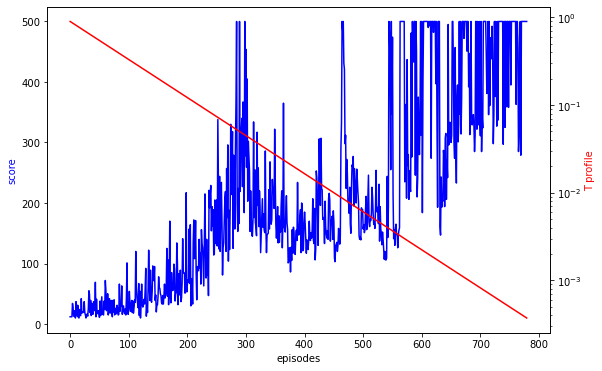
\includegraphics[width=0.45\textwidth]{img/vanilla2.png}} \quad
    \subfloat[$w_x=-0.2, e_x=4, w_\theta=-5, e_\theta=4$]{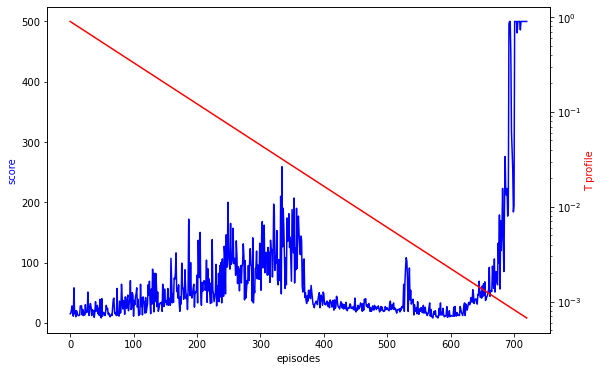
\includegraphics[width=0.45\textwidth]{img/mod_r_cv.png}} \\
    \subfloat[Wavy]{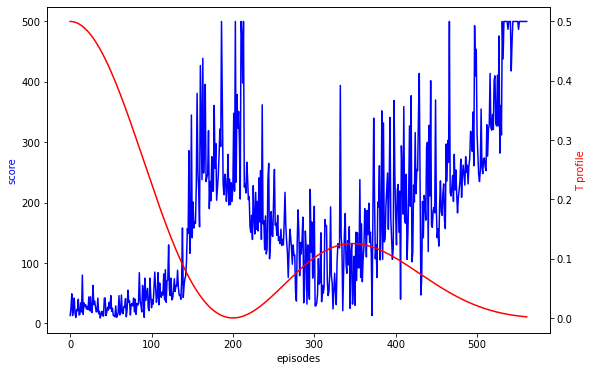
\includegraphics[width=0.45\textwidth]{img/wavy3.png}} \quad
    \subfloat[Best]{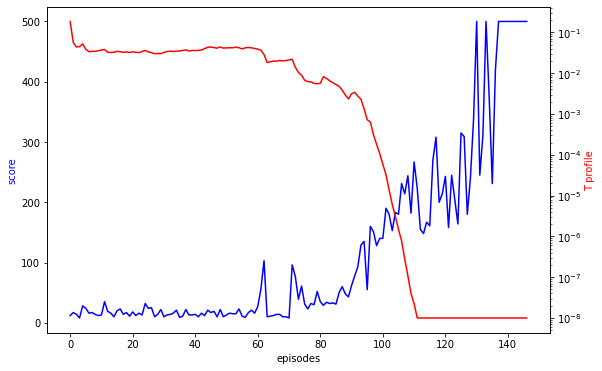
\includegraphics[width=0.45\textwidth]{img/best.png}}
    \caption{Behavior of the agent score and the softmax temperature during learning for four different cases.}
    \label{fig:scores}
  \end{figure}





\section{Cart-Pole with screen pixels}

\section{Other gym env}





\end{document}
